\documentclass[11pt,a4paper]{article}
\usepackage[utf8x]{inputenc}
\usepackage[T1]{fontenc}
\usepackage{mathptmx}
\usepackage{graphicx}
\usepackage[pdftex,linkcolor=black,pdfborder={0 0 0}]{hyperref} % Format links for pdf
\usepackage{calc} % To reset the counter in the document after title page
\usepackage{enumitem} % Includes lists
\usepackage{caption}
\captionsetup[figure]{font=small,labelfont=small,labelfont=bf}
\usepackage{subcaption}
\usepackage{amsmath}
\usepackage{amssymb}
\usepackage{amsfonts}
\usepackage{fancyvrb,newverbs,xcolor}
\usepackage{verbatim}
\definecolor{cverbbg}{gray}{0.93}

\newenvironment{lcverbatim}
 {\SaveVerbatim{cverb}}
 {\endSaveVerbatim
  \flushleft\fboxrule=0pt\fboxsep=.5em
  \colorbox{cverbbg}{%
    \makebox[\dimexpr\linewidth-2\fboxsep][l]{\BUseVerbatim{cverb}}%
  }
  \endflushleft
}

\renewcommand\thesection{Task \arabic{section}}
\renewcommand\thesubsection{\alph{subsection}.)}
\renewcommand\thesubsubsection{\Roman{subsubsection}:}

\frenchspacing
\linespread{1.2}
\usepackage[a4paper, lmargin=0.12\paperwidth, rmargin=0.12\paperwidth, tmargin=0.05\paperheight, bmargin=0.1\paperheight]{geometry}

\usepackage[all]{nowidow} % Tries to remove widows
\usepackage[protrusion=true,expansion=true]{microtype}

\title{Exercise 6}
\author{Kai Schneider}
\date{\today}

\begin{document} 

\maketitle

\section{Planning and Learning}

\subsection{}

\begin{itemize}
  \item In the first phase Dyna-Q+ performs better due to the additional reward given by exploring the environment
  \item After changing the environment, Dyna-Q+ still performs better because it keeps on exploring and thus is able to find
  the new shortcut. In contrast, Dyna-Q is unable to find the shorter path because the already trained Q-function always chooses
  the "left" path. This way the reward rate stays the same, while the one of Dyna-Q+ increases after a certain time.
\end{itemize}
Dyna-Q+ improves exploring the environment as well as adapting to changing circumstances.

\subsection{}

In an stochastic environment the agent can't determine transition and reward completely because it isn't deterministic\\
One solution to this problem would be to keep track of the rewards given by die $(s,a)$-pairs in the environment in form of 
probabilities ($\sim P(r|s,a,s')$). We than can use this information during the planning phase.\\
If our environment is not only non-deterministic, but also changing, this method could be problematic. Our "old" probabilities
would no longer be useful for approximating our real environment. A solution could be some sort of decay to "forget" too old data. 
By using only a few newer samples instead of the whole data for calculating our probabilities we can adapt to a changing environment.

\newpage

\section{}

\subsection{}
\begin{figure}[!h]
  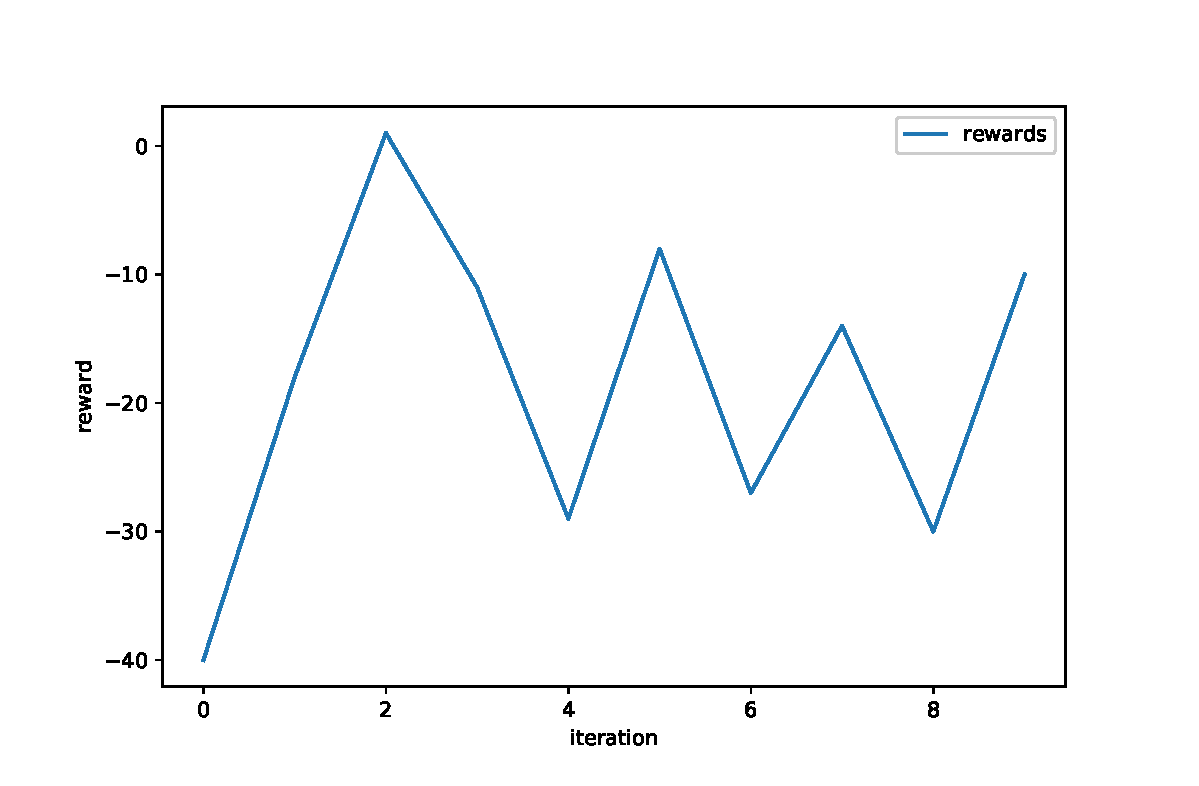
\includegraphics[width=.7\textwidth]{reward.eps}
  \centering
  \caption{average reward over the iterations}
  \label{fig1}
\end{figure}

\subsection{}

\begin{figure}[h!]
  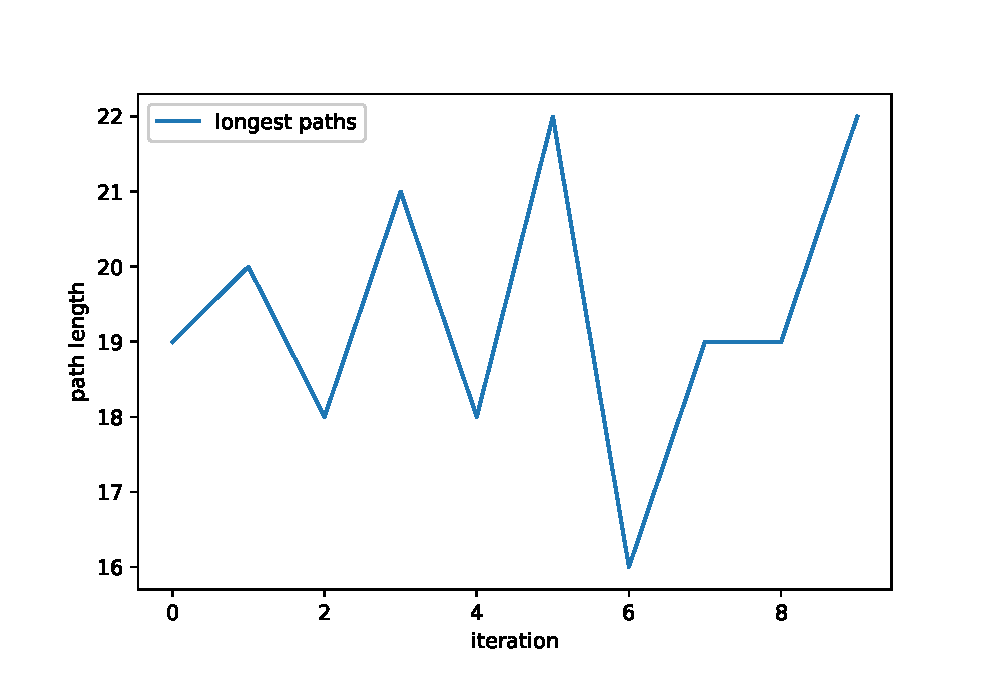
\includegraphics[width=.7\textwidth]{path_length.eps}
  \centering
  \caption{plot of length of the longest path over the iterations}
  \label{fig2}
\end{figure}



\end{document}

